
\medskip  

\parbox{0.78\linewidth}{Le maraîchage est l'activité professionnelle qui consiste à cultiver les légumes, certains fruits, fleurs ou plantes aromatiques.

Afin de diminuer la pénibilité des travaux de maraîchage, un agriculteur a
acquis un robot électrique pour effectuer le désherbage de ses cultures.}\hfill
\parbox{0.2\linewidth}{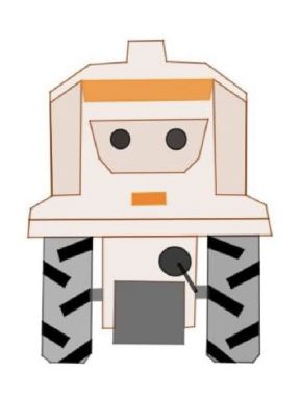
\includegraphics[width=3cm]{robot}}

\bigskip

\textbf{Partie A. Parcours du robot}

\medskip

Le robot doit parcourir 49 allées parallèles écartés de 1~m, représentées sur le schéma ci-dessous.

Les 48 premières allées, situées dans une parcelle rectangulaire, mesurent 80 m de long:

\setlength\parindent{4mm}
\begin{itemize}
\item[$\bullet~$] la 1\up{re} allée est [PQ] ; 
\item[$\bullet~$] la 2\up{e} allée est [RS] ; 
\item[$\bullet~$] la 3\up{e} allée est [TU] ; 
\item[$\bullet~$] les allées 4 à 47 ne sont pas représentées ; 
\item[$\bullet~$] la 48\up{e} allée est [CB]. 
\end{itemize}
\setlength\parindent{0mm}

la 49\up{e} (dernière allée) [DE] est située dans une parcelle triangulaire.

\medskip
 
Montrer que la longueur de la dernière allée est  DE $= 64$~m. 
\begin{center}
\psset{unit=1cm}
\begin{pspicture}(0,-1)(8,6)
%\psgrid 
\def\barbar{\psline(-0.1,-0.05)\psline(0.1,-0.05)\psline(-0.1,0.05)
\psline(0.1,0.05)}
\psframe(1,1)(2.6,5)
\psline(4,5)(7,1)(4,1)
\psline(1.8,1)(1.8,5)  \psline(2.6,1)(2.6,5) %\psline(3.4,1)(3.4,5) 
\psline(4.8,1)(4.8,3.95)
\psline(4,1)(4,5)%CB 
\psline[linestyle=dotted](4,5)(2.6,5)
\psline[linestyle=dotted](4,1)(2.6,1)
\psline[linewidth=0.5pt]{<->}(0.5,1)(0.5,5)\uput[l](0.5,3){80~m}
\psline[linewidth=0.5pt]{<->}(4,0.5)(7,0.5)\uput[d](5.5,0.5){5~m}
\rput(1,3){\barbar}\rput(1.8,3){\barbar}
\rput(2.6,3){\barbar}%\rput(3.4,3){\barbar}
\uput[dl](1,1){P} \uput[d](1.8,1){S} \uput[d](2.6,1){T} \uput[d](4,1){B} 
\uput[d](4.8,1){D} \uput[d](7,1){F} \uput[ur](4.8,3.95){E} \uput[u](4,5){C} 
\uput[u](2.6,5){U} \uput[u](1.8,5){R} \uput[ul](1,5){Q}
\rput(6.1,3.8){(BC) // (DE)}
\rput(1.4,4.5){\tiny salade}\psline[linestyle=dotted](1.4,4.25)(1.4,1.75)
\rput(2.14,4.5){\tiny salade}\rput(2.14,1.5){\tiny salade}
\rput(1.4,1.5){\tiny salade}\rput(4.475,1.5){\tiny salade}\rput(4.475,4){\tiny salade}
\psline[linestyle=dotted](1.4,4.25)(1.4,1.75)
\psline[linestyle=dotted](2.2,4.25)(2.2,1.75)
\psline[linestyle=dotted](4.475,3.8)(4.475,1.75)
\psline(1.4,1.1)(1.4,0.9)\psline(2.2,1.1)(2.2,0.9)\psline(4.4,1.1)(4.4,0.9)
\psline(1.4,5.1)(1.4,4.9)\psline(2.2,5.1)(2.2,4.9)
\uput[u](4.4,1){1~m}
\rput(4,-0.25){Schéma 2 du terrain non à l'échelle:}
\rput(4,-0.75){vue du dessus}
\end{pspicture}
\end{center}

\bigskip

\textbf{Partie B. Programme de déplacement du robot}

On souhaite programmer le déplacement du robot du point P au point E. Le script ci-dessous,
réalisé sous Scratch, est incomplet. Toutes les allées sont parcourues une seule fois. L'image\og Robot\fg correspond au résultat attendu lorsque le drapeau vert est cliqué.

\smallskip

On rappelle que l'instruction \begin{scratch}\blockmove{s’orienter à \ovalnum{0\selectarrownum} degrés}\end{scratch} signifie que le robot se dirige vers le haut.

\medskip

\begin{tabularx}{\linewidth}{|*3{X}|}\hline
\begin{scratch}
\blockinit{Quand \greenflag est cliqué}
\blockmove{s’orienter à \ovalnum{0\selectarrownum}}
\blockpen{stylo en position d’écriture}
\blockrepeat{répéter \ovalnum{x} fois}
{
\blockmoreblocks{Motif montant}
\blockmoreblocks{Motif descendant}
}
\blockmove{avancer de \ovalnum{y}}
\blockpen{relever le stylo}
\end{scratch}&
\begin{scratch}
\initmoreblocks{définir \namemoreblocks{Motif montant}}
\end{scratch}

\medskip

\begin{scratch}
\initmoreblocks{définir \namemoreblocks{Motif descendant}}
\end{scratch}&Robot \hfill \pscircle[fillstyle=solid,fillcolor=red](0,0){0.25cm}

\begin{pspicture}(4,6)
\psset{unit=1cm}
\multido{\n=0.0+0.15}{26}{\psline(\n,0.1)(\n,5.7)}
\multido{\n=0.0+0.3,\na=0.15+0.30}{13}{\psline(\n,5.7)(\na,5.7)}
\multido{\n=0.15+0.30,\na=0.30+0.30}{13}{\psline(\n,0.1)(\na,0.1)}
\rput(4.1,0.5){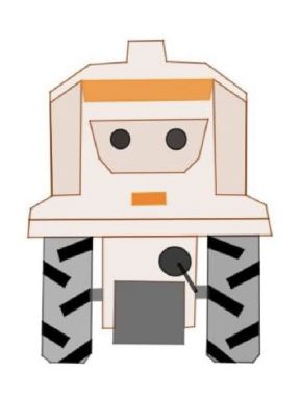
\includegraphics[width=0.5cm]{robot}}
\end{pspicture}\\
\multicolumn{2}{c}{Script incomplet de déplacement du robot}&~\\
\multicolumn{2}{r}{Image à obtenir avec le script complet $\to$}&~\\ \hline
\end{tabularx}

\medskip

Pour répondre aux questions 1 et 2, utiliser autant que nécessaire les blocs:

\begin{center}\begin{scratch}\blockmove{avancer de \ovalnum{}}\end{scratch} \:\begin{scratch}\blockmove{tourner \turnright{} de \ovalnum{} degrés} \end{scratch} \:\begin{scratch}\blockmove{tourner \turnleft{} de \ovalnum{} degrés}\end{scratch}\end{center}

Les longueurs doivent être indiquées en mètres.

\medskip

\begin{enumerate}
\item Le nouveau bloc \og Motif montant \fg{} doit reproduire un déplacement du type P--Q--R (voir schéma 2) et positionner le robot prêt à réaliser le motif suivant. 

Écrire une succession de 4 blocs permettant de définir : \og Motif montant \fg.
\item Le nouveau bloc \og Motif descendant\fg{} doit reproduire un déplacement du type R--S--T (voir schéma 2) et positionner le robot prêt à réaliser le motif suivant.

Quelle(s) modification(s) suffit-il d'apporter au bloc \og Motif montant\fg{} pour obtenir le bloc \og Motif descendant\fg{} ?
\item Quelles valeurs faut-il donner à $x$ et à $y$ dans le script principal pour que le programme de déplacement du robot donne le résultat attendu.
\end{enumerate}




